\newpage
\section{Tables}
\renewcommand{\thetable}{\thesection \arabic{table}}
\setcounter{table}{0}

\begingroup
\setlength{\tabcolsep}{4pt}
\renewcommand{\arraystretch}{0.95}
  \begin{table}
  \centering
  \begin{tabular}{rcc|rr|rr}
  \toprule
  Year & \multicolumn{2}{c|}{Consumer Price Index} & \multicolumn{2}{c|}{Average Payout (EUR)} & \multicolumn{2}{c}{Financial Expenditure (EUR 1,000)} \\
  \cmidrule(lr){2-3} \cmidrule(lr){4-5} \cmidrule(l){6-7}
  & Index (2020=100) & Price Factor (2023) & Nominal & Real (2023) & Nominal & Real (2023) \\
  \midrule
  1991 & 61 & 1.885 & 290 & 547 & 1,538,590 & 2,900,701 \\
  1992 & 65 & 1.795 & 290 & 521 & 1,539,929 & 2,764,764 \\
  1993 & 67 & 1.719 & 297 & 510 & 1,458,164 & 2,506,152 \\
  1994 & 69 & 1.674 & 295 & 494 & 1,257,002 & 2,104,621 \\
  1995 & 71 & 1.644 & 304 & 500 & 1,133,989 & 1,863,894 \\
  1996 & 72 & 1.621 & 322 & 522 & 1,059,270 & 1,716,900 \\
  1997 & 73 & 1.590 & 319 & 507 & 910,038 & 1,446,886 \\
  1998 & 74 & 1.577 & 316 & 498 & 861,688 & 1,358,905 \\
  1999 & 74 & 1.566 & 321 & 503 & 871,140 & 1,364,591 \\
  2000 & 75 & 1.546 & 326 & 504 & 906,857 & 1,401,724 \\
  2001 & 77 & 1.516 & 365 & 553 & 1,161,922 & 1,760,990 \\
  2002 & 78 & 1.494 & 371 & 554 & 1,350,543 & 2,018,032 \\
  2003 & 78 & 1.479 & 370 & 547 & 1,446,120 & 2,138,937 \\
  2004 & 80 & 1.455 & 371 & 540 & 1,513,641 & 2,202,517 \\
  2005 & 81 & 1.432 & 375 & 537 & 1,554,602 & 2,226,037 \\
  2006 & 82 & 1.409 & 375 & 529 & 1,538,770 & 2,168,773 \\
  2007 & 84 & 1.378 & 375 & 517 & 1,490,718 & 2,053,917 \\
  2008 & 86 & 1.343 & 398 & 534 & 1,590,638 & 2,136,104 \\
  2009 & 87 & 1.338 & 434 & 581 & 1,875,731 & 2,510,295 \\
  2010 & 88 & 1.325 & 436 & 578 & 2,019,078 & 2,674,533 \\
  2011 & 90 & 1.297 & 452 & 586 & 2,269,706 & 2,943,052 \\
  2012 & 91 & 1.273 & 448 & 570 & 2,364,963 & 3,009,718 \\
  2013 & 93 & 1.253 & 446 & 559 & 2,349,400 & 2,944,951 \\
  2014 & 94 & 1.241 & 448 & 556 & 2,280,748 & 2,831,524 \\
  2015 & 94 & 1.235 & 448 & 553 & 2,157,634 & 2,664,506 \\
  2016 & 95 & 1.228 & 464 & 570 & 2,099,110 & 2,578,590 \\
  2017 & 96 & 1.211 & 499 & 604 & 2,181,049 & 2,640,336 \\
  2018 & 98 & 1.190 & 493 & 586 & 2,001,732 & 2,381,265 \\
  2019 & 99 & 1.173 & 514 & 603 & 1,954,449 & 2,292,303 \\
  2020 & 100 & 1.167 & 574 & 670 & 2,210,920 & 2,580,143 \\
  2021 & 103 & 1.132 & 579 & 655 & 2,316,926 & 2,622,553 \\
  2022 & 110 & 1.059 & 611 & 647 & 2,454,392 & 2,599,161 \\
  2023 & 116 & 1.000 & 663 & 663 & 2,863,514 & 2,863,514 \\
  \bottomrule
  \end{tabular}
  \caption{
    Average nominal and inflation-adjusted payout under the Federal Training Assistance Act (BAföG) 
    for student recipients (excluding pupils), based on official data published by Destatis.  
    The table includes the Consumer Price Index (CPI, variable \textbf{PREIS1}, base year 2020 = 100) and 
    a derived price factor (column “Factor (2023)”) calculated using these CPI values to express nominal amounts in 2023 euros.  
    The inflation-adjusted average payouts and total financial expenditures were computed using this deflator and are not 
    reported as such in the original Destatis tables.
  }
  \label{table:payout_over_time}
  \end{table}
\endgroup

\begin{landscape}
\setlength{\tabcolsep}{4pt} % horizontal spacing between columns
\renewcommand{\arraystretch}{0.95} % vertical spacing between rows
\begin{table}
\centering
\begin{tabular}{rrrrrrrr}
\toprule
Year & Students & \multicolumn{3}{|c|}{Number of Supported Students} & \multicolumn{3}{c}{Proportion Supported (\%)} \\
\midrule
 & & Total Supported & Fully Supported & Partially Supported & Total & Fully & Partially \\
\midrule
2023 & 2,868,311 & 501,425 & 245,255 & 256,170 & 17.5 & 8.6 & 8.9 \\
2022 & 2,920,263 & 489,347 & 244,559 & 244,788 & 16.8 & 8.4 & 8.4 \\
2021 & 2,941,915 & 467,595 & 200,369 & 267,226 & 15.9 & 6.8 & 9.1 \\
2020 & 2,944,145 & 465,543 & 205,093 & 260,450 & 15.8 & 7.0 & 8.8 \\
2019 & 2,891,049 & 489,313 & 212,217 & 277,096 & 16.9 & 7.3 & 9.6 \\
2018 & 2,868,222 & 517,675 & 218,427 & 299,248 & 18.0 & 7.6 & 10.4 \\
2017 & 2,844,978 & 556,573 & 229,053 & 327,520 & 19.6 & 8.1 & 11.5 \\
2016 & 2,807,010 & 583,567 & 235,163 & 348,404 & 20.8 & 8.4 & 12.4 \\
2015 & 2,757,799 & 611,377 & 231,477 & 379,900 & 22.2 & 8.4 & 13.8 \\
2014 & 2,698,910 & 646,576 & 246,901 & 399,675 & 24.0 & 9.1 & 14.8 \\
2013 & 2,616,881 & 665,928 & 253,371 & 412,557 & 25.4 & 9.7 & 15.8 \\
2012 & 2,499,409 & 671,042 & 254,769 & 416,273 & 26.8 & 10.2 & 16.7 \\
2011 & 2,380,974 & 643,578 & 246,895 & 396,683 & 27.0 & 10.4 & 16.7 \\
2010 & 2,217,294 & 592,430 & 232,796 & 359,633 & 26.7 & 10.5 & 16.2 \\
2009 & 2,121,178 & 550,369 & 211,881 & 338,488 & 25.9 & 10.0 & 16.0 \\
2008 & 2,025,307 & 510,409 & 217,933 & 292,476 & 25.2 & 10.8 & 14.4 \\
2007 & 1,941,405 & 494,480 & 191,268 & 303,212 & 25.5 & 9.9 & 15.6 \\
2006 & 1,979,043 & 498,565 & 189,022 & 309,543 & 25.2 & 9.6 & 15.6 \\
2005 & 1,985,765 & 506,880 & 193,285 & 313,595 & 25.5 & 9.7 & 15.8 \\
2004 & 1,963,108 & 497,257 & 186,956 & 310,301 & 25.3 & 9.5 & 15.8 \\
2003 & 2,019,465 & 481,594 & 179,755 & 301,839 & 23.8 & 8.9 & 14.9 \\
2002 & 1,938,811 & 451,505 & 168,890 & 282,615 & 23.3 & 8.7 & 14.6 \\
2001 & 1,868,331 & 406,776 & 134,933 & 271,843 & 21.8 & 7.2 & 14.6 \\
2000 & 1,798,863 & 348,799 & 100,913 & 247,886 & 19.4 & 5.6 & 13.8 \\
1999 & 1,770,489 & 338,427 & 103,239 & 235,188 & 19.1 & 5.8 & 13.3 \\
1998 & 1,800,651 & 336,355 & 97,539 & 238,810 & 18.7 & 5.4 & 13.3 \\
\bottomrule
\end{tabular}
\caption{
  Number and percentage of students receiving BAföG support.  
  Columns:  
  \textbf{BIL002} = total number of students;  
  \textbf{PER010} = total supported students;  
  \textbf{PER011} = fully supported students;  
  \textbf{PER012} = partially supported students.
}
\label{table:bafoeg_support_landscape}
\end{table}
\end{landscape}

% # Variable codes 
% # PER 010 | Supported persons
% # PER 011 | Persons receiving full assistance payments
% # PER 012 | Persons receiving partial assistance payments
% # PER 013 | Supported persons (average monthly stock)
% # PER 014 | Average monthly assistance payment per person




\begin{landscape}
\begin{table}[htbp]
\centering
\label{tab:nontakeup_hgtyp_migback_sex_east_siblings}
\begin{tabular}{lccccccccccccccc}
\toprule
Household Type & 2007 & 2008 & 2009 & 2010 & 2011 & 2012 & 2013 & 2014 & 2015 & 2016 & 2017 & 2018 & 2019 & 2020 & 2021 \\
\midrule
1-Person Household      & 52.38 & 52.38 & 64.71 & 72.22 & 60.00 & 38.71 & 41.18 & 37.93 & 56.00 & 55.56 & 46.67 & 64.29 & 54.55 & 59.38 & 63.33 \\
Couple Without Children & 80.00 & 50.00 & 75.00 & 100.00 & 75.00 & 50.00 & 63.64 & 88.89 & 36.36 & 85.71 & 69.23 & 46.15 & 60.00 & 90.00 & 71.43 \\
Couple With Children    & 66.67 & 70.83 & 56.86 & 56.86 & 51.90 & 56.96 & 51.69 & 59.49 & 71.43 & 53.13 & 66.67 & 66.67 & 73.24 & 67.27 & 77.27 \\
\midrule
Migration Background & 2007 & 2008 & 2009 & 2010 & 2011 & 2012 & 2013 & 2014 & 2015 & 2016 & 2017 & 2018 & 2019 & 2020 & 2021 \\
\midrule
No migration background   & 61.22 & 64.41 & 66.10 & 65.08 & 53.33 & 53.47 & 52.44 & 59.04 & 65.85 & 62.32 & 67.39 & 63.04 & 67.11 & 63.29 & 65.43 \\
With migration background & 58.82 & 61.54 & 47.83 & 50.00 & 54.76 & 45.71 & 46.67 & 49.06 & 60.47 & 47.83 & 54.55 & 65.46 & 68.42 & 64.71 & 70.00 \\
\midrule
Sex & 2007 & 2008 & 2009 & 2010 & 2011 & 2012 & 2013 & 2014 & 2015 & 2016 & 2017 & 2018 & 2019 & 2020 & 2021 \\
\midrule
Male   & 68.97 & 69.44 & 58.54 & 69.23 & 50.00 & 53.73 & 47.89 & 53.52 & 61.91 & 64.00 & 70.31 & 64.79 & 64.29 & 58.33 & 68.00 \\
Female & 54.05 & 59.18 & 63.42 & 54.17 & 56.94 & 49.28 & 52.11 & 56.92 & 66.13 & 50.77 & 56.63 & 63.16 & 70.69 & 67.69 & 65.57 \\
\midrule
Region & 2007 & 2008 & 2009 & 2010 & 2011 & 2012 & 2013 & 2014 & 2015 & 2016 & 2017 & 2018 & 2019 & 2020 & 2021 \\
\midrule
West Germany & 73.17 & 69.70 & 67.21 & 62.50 & 56.70 & 59.14 & 50.00 & 59.63 & 67.00 & 62.22 & 67.80 & 67.23 & 70.97 & 71.11 & 72.62 \\
East Germany & 40.00 & 42.11 & 42.86 & 56.52 & 45.71 & 34.88 & 50.00 & 37.04 & 52.00 & 36.00 & 41.38 & 50.00 & 52.38 & 34.78 & 48.15 \\
\midrule
Sibling BAföG history & 2007 & 2008 & 2009 & 2010 & 2011 & 2012 & 2013 & 2014 & 2015 & 2016 & 2017 & 2018 & 2019 & 2020 & 2021 \\
\midrule
No sibling received BAföG & 65.52 & 63.33 & 53.85 & 60.87 & 64.87 & 61.29 & 56.76 & 73.17 & 58.97 & 72.41 & 70.27 & 52.50 & 75.68 & 66.67 & 63.33 \\
Sibling received BAföG    & 61.54 & 64.71 & 46.15 & 53.33 & 48.48 & 32.14 & 37.50 & 56.00 & 68.18 & 44.44 & 44.74 & 63.64 & 60.00 & 43.75 & 55.56 \\
\bottomrule
\end{tabular}
\caption{Non-take-up rates by household type, migration background, sex, region, number of siblings, and sibling BAföG history.}
\end{table}
\end{landscape}


\begin{figure}[htbp]
  \centering
  \begin{subfigure}[t]{0.48\linewidth}
    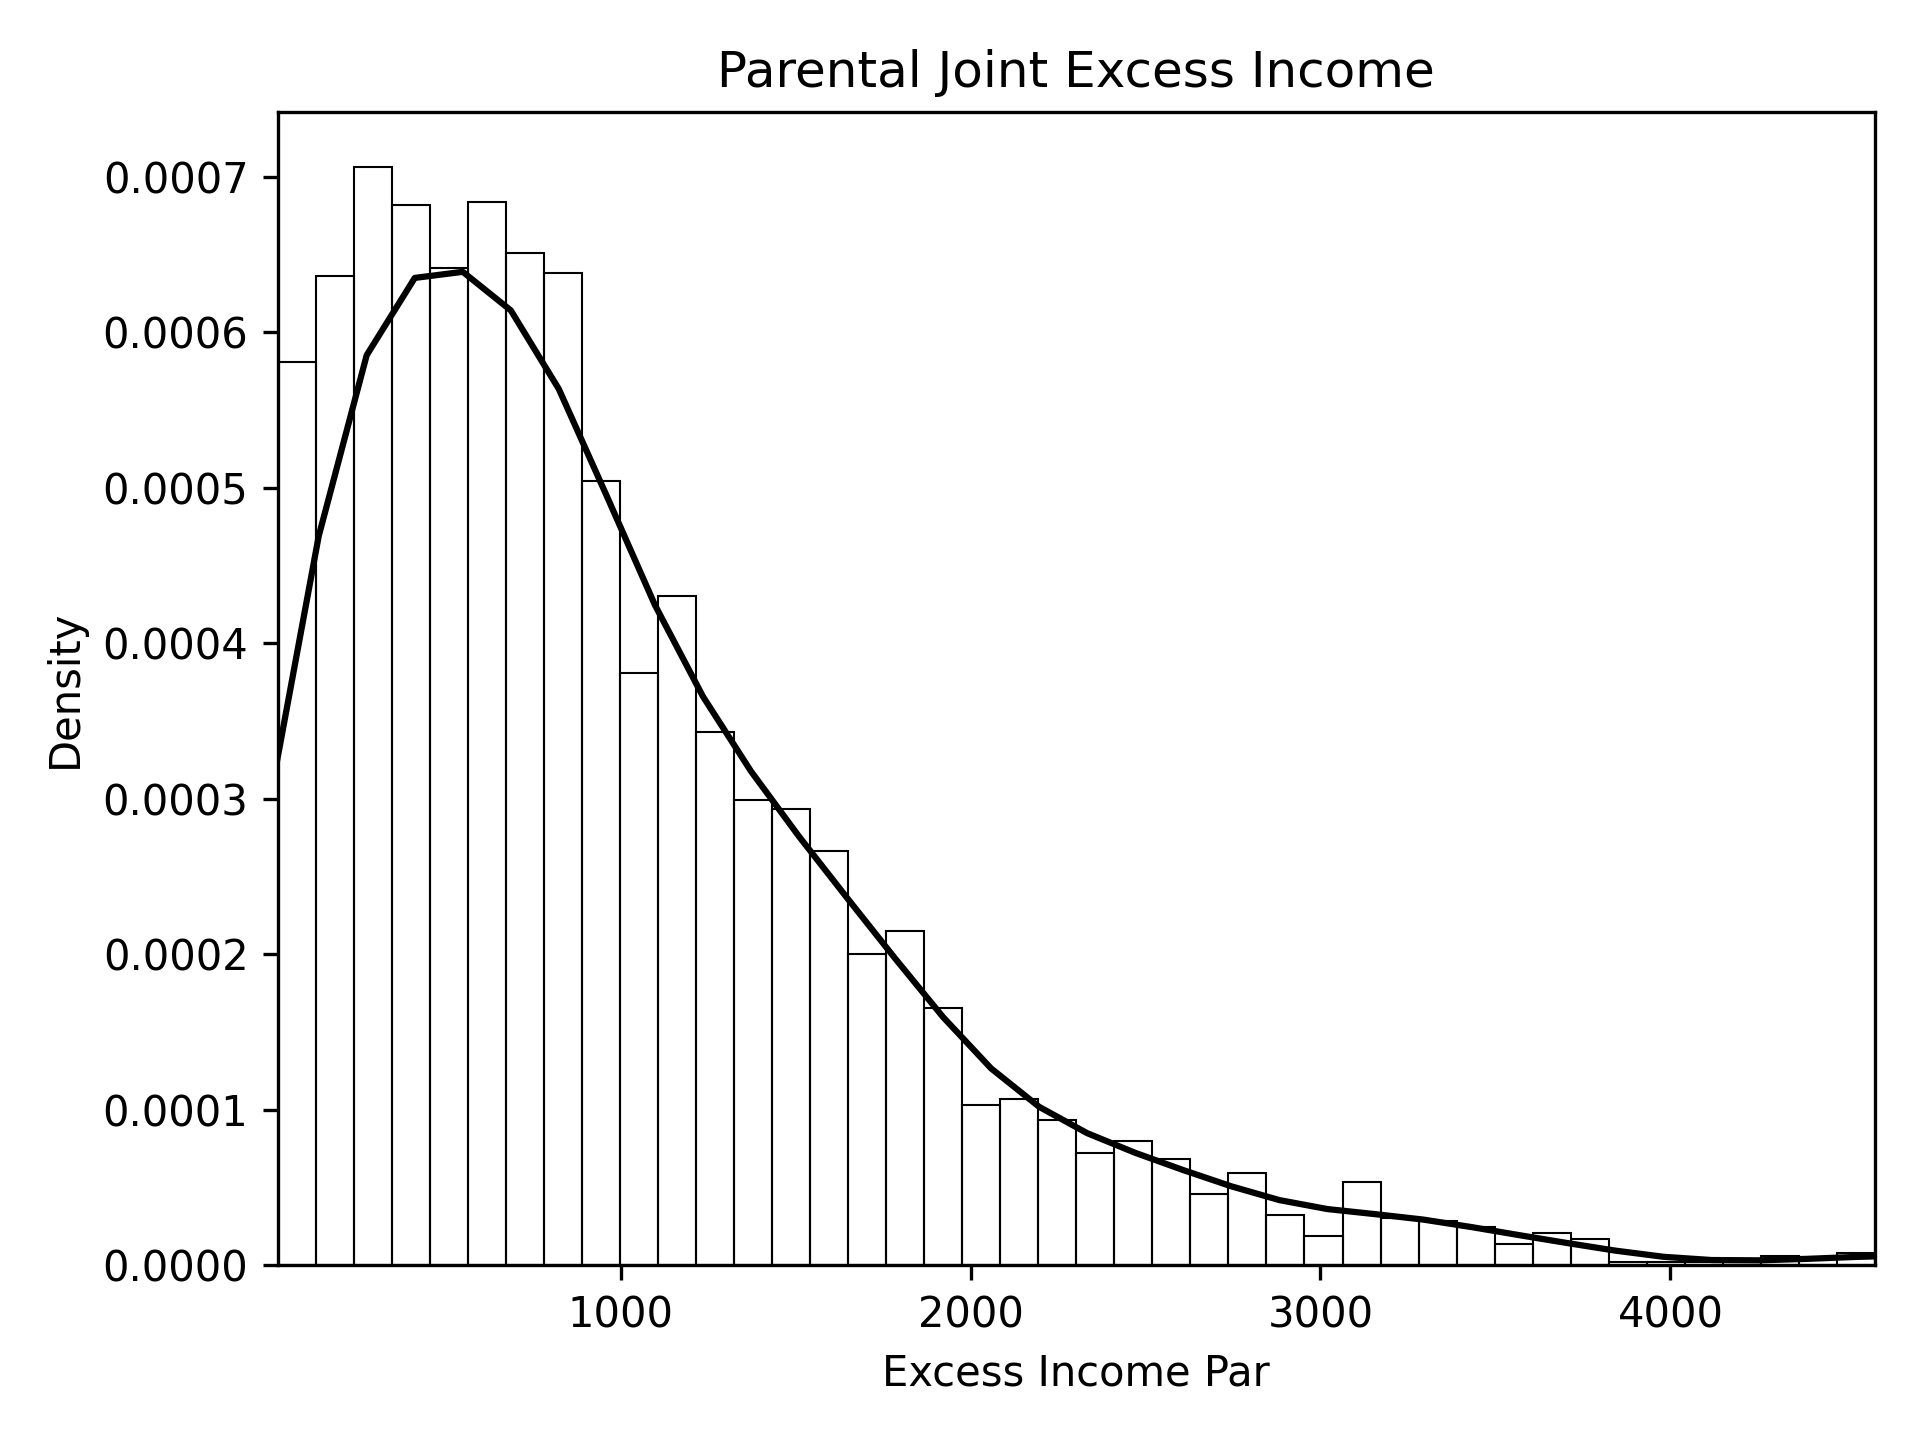
\includegraphics[width=\linewidth]{parental_joint_excess_income_pdf.png}
    \caption{Parental joint excess income}
    \label{fig:parental-excess}
  \end{subfigure}
  \hfill
  \begin{subfigure}[t]{0.48\linewidth}
    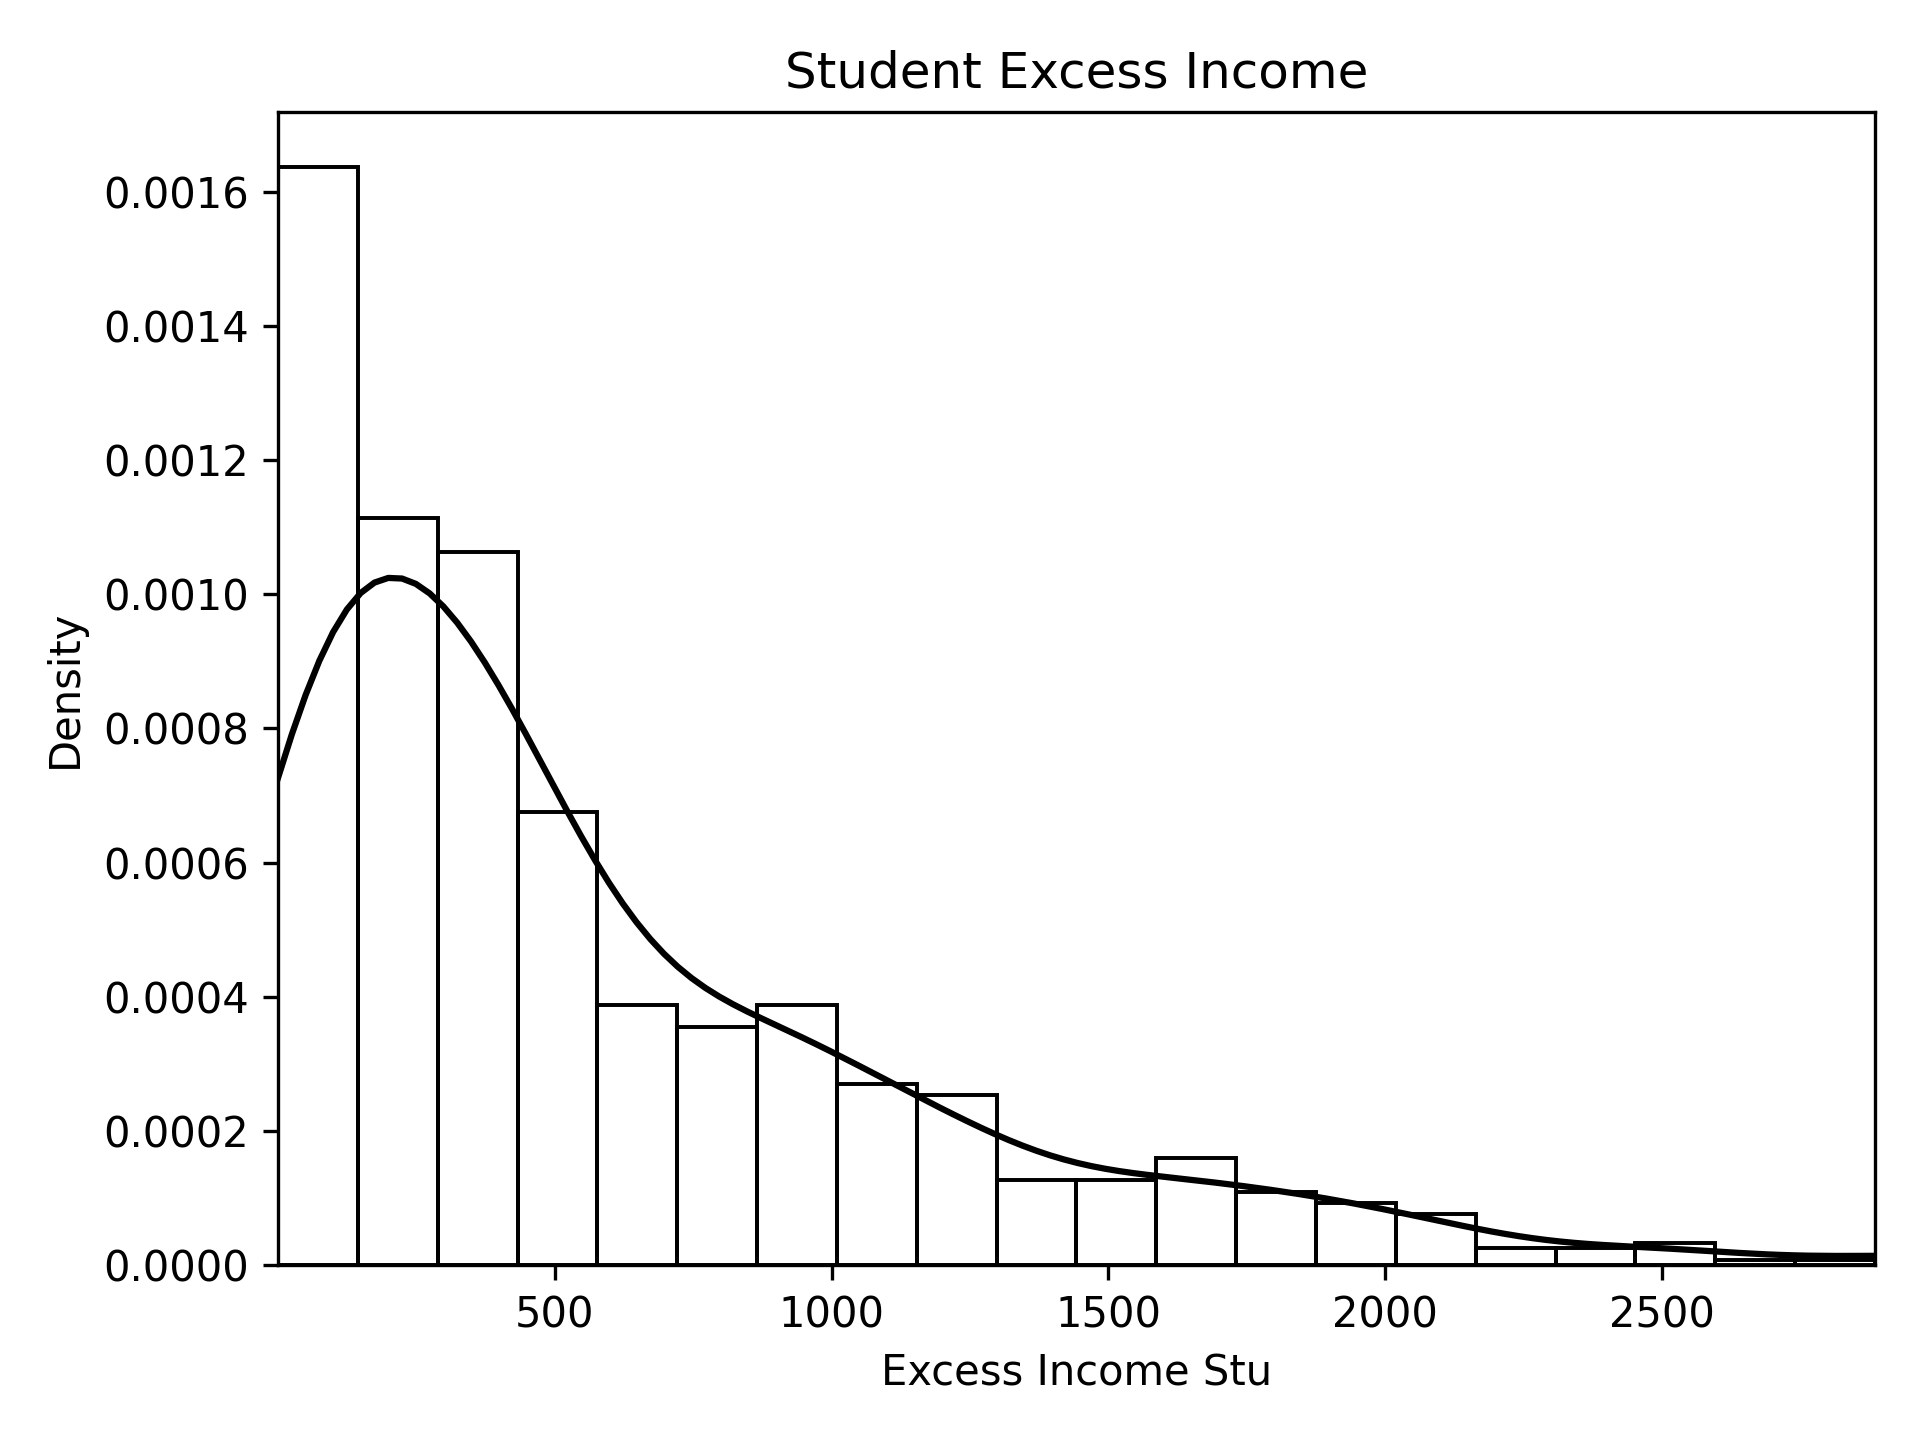
\includegraphics[width=\linewidth]{student_excess_income_pdf.png}
    \caption{Student excess income}
    \label{fig:student-excess}
  \end{subfigure}
  \caption{Simulated mean excess income for parents (\subref{fig:parental-excess}) and students (\subref{fig:student-excess}).}
  \label{fig:excess-income}
\end{figure}


\begin{figure}[htbp]
  \centering
  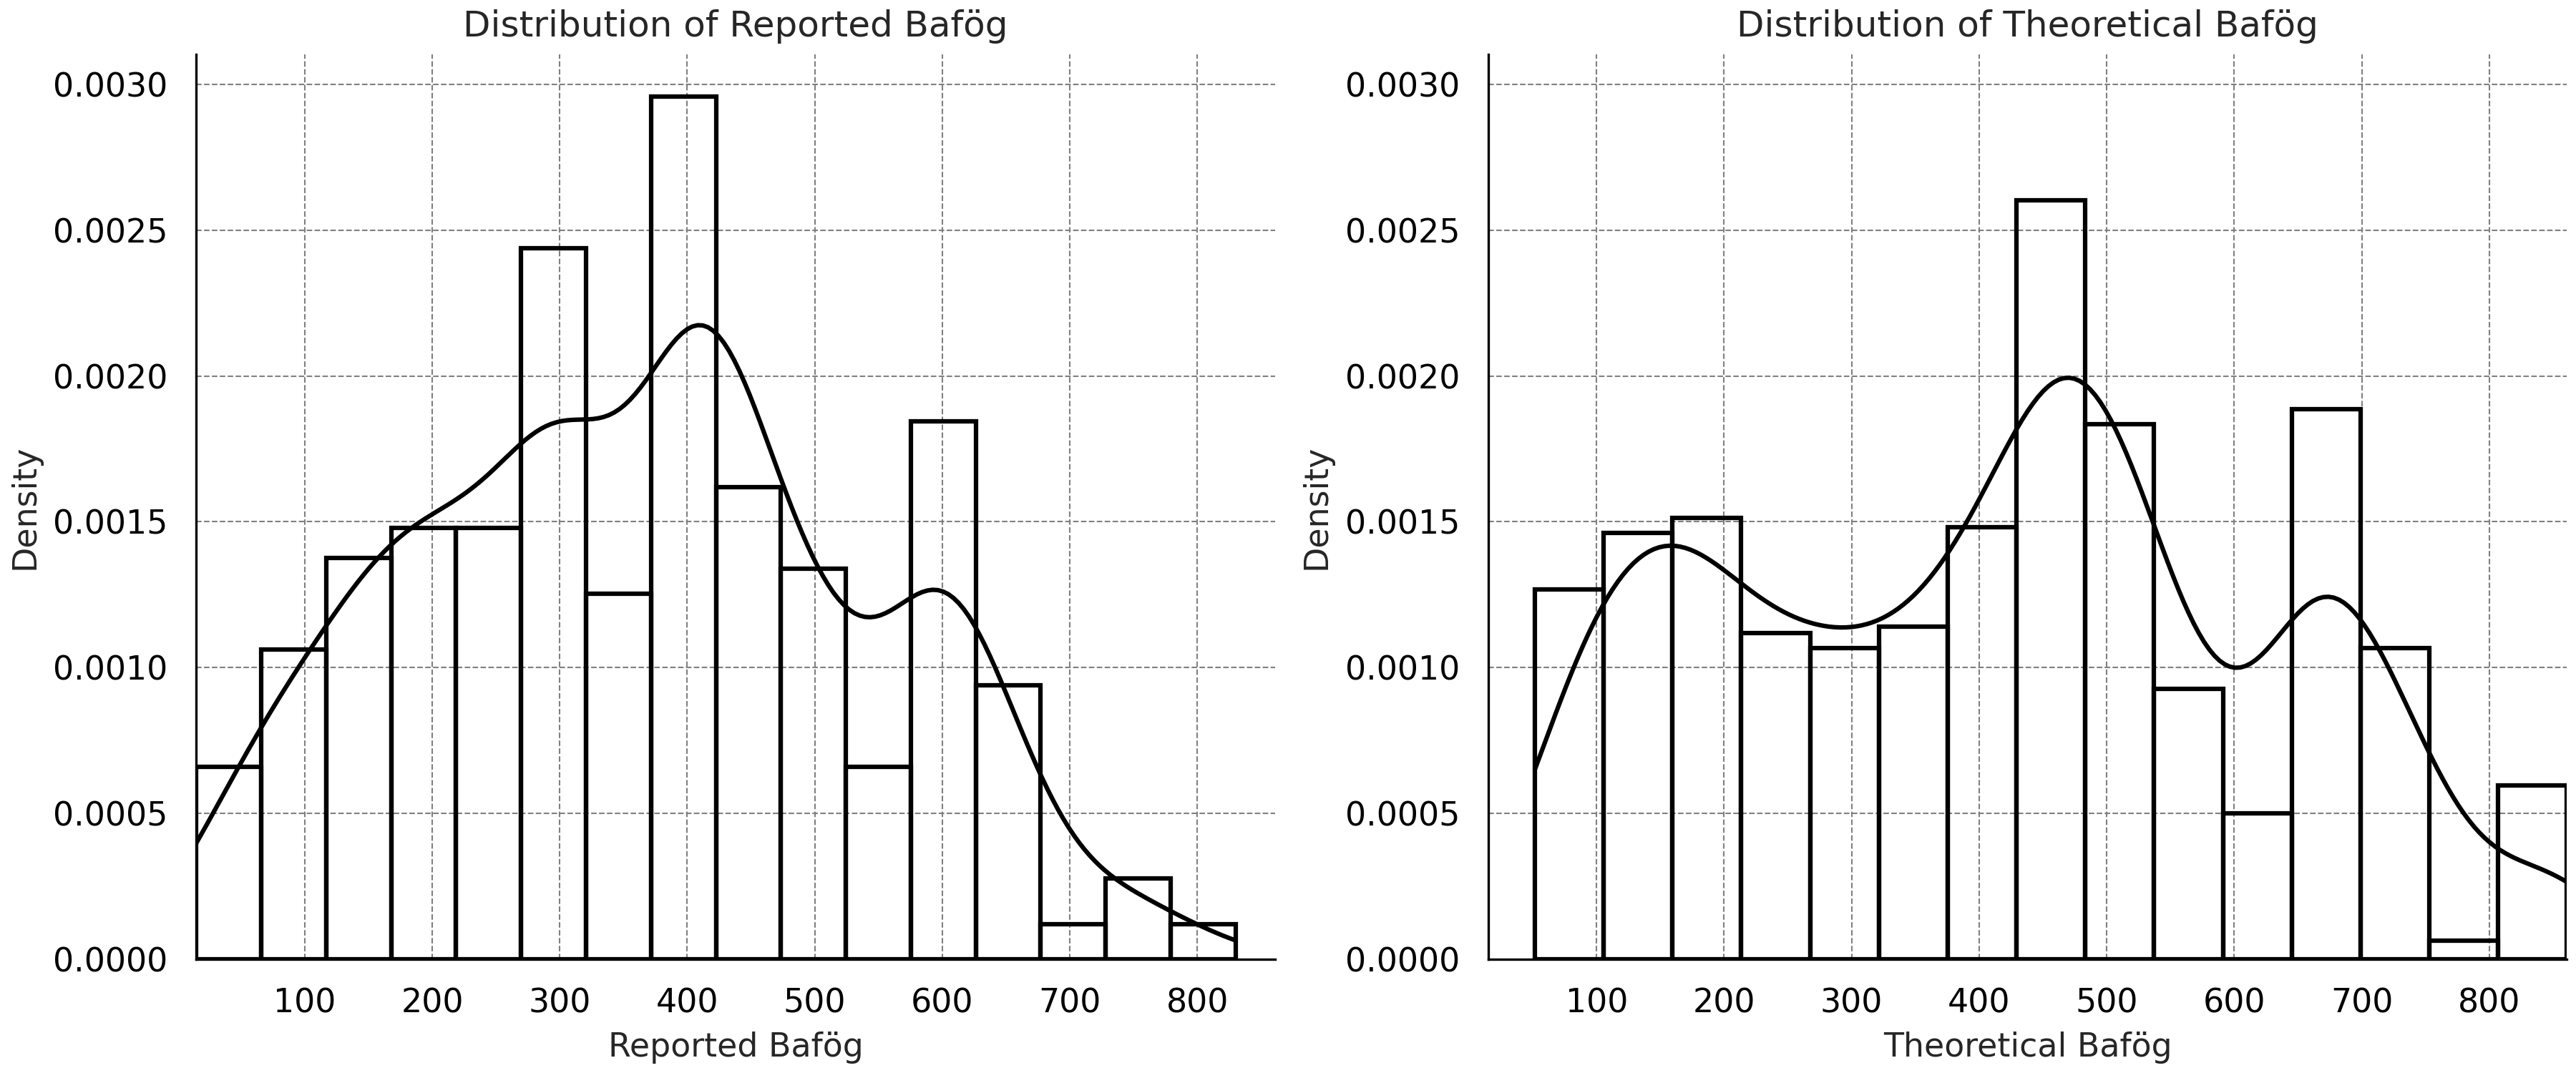
\includegraphics[width=0.95\linewidth]{theo_vs_reported_distribution.png}
  \caption{Comparison of the distribution of reported BAföG receipt in the SOEP-Core sample with the simulated (theoretical) distribution of simulated BAföG entitlements from our model.}
  \label{fig:theo-vs-reported}
\end{figure}
